%本論

\documentclass[11pt, a4paper]{jarticle}
\usepackage[dvipdfmx]{graphicx}
\usepackage[divpdfm]{graphicx}
\usepackage[dvipdfmx]{hyperref}
\usepackage{ascmac}
\usepackage{listings}
\usepackage{fancyhdr}
\usepackage{pxjahyper}

%余白設定
\setlength{\textwidth}{455pt}
\setlength{\hoffset}{5truemm}
\addtolength{\textwidth}{-25truemm}

%行間の倍率
\renewcommand{\baselinestretch}{1.0}

%maketitleの編集
\makeatletter
  \def\@maketitle{%
    \clearpage\null
    \begin{center}%
      \vskip 10.0em
      \let\footnote\thanks
      {\LARGE \@title \par}%
      \vskip 4.0em
      {\Large
        \lineskip 0.5em
        \begin{tabular}[t]{c}%
          \@author
        \end{tabular}\par}%
      \vskip 3.0em
      {\Large \@date}%
    \end{center}%
    \par\vskip 0.5em
    \ifvoid\@abstractbox\else\centerline{\box\@abstractbox}\vskip1.5em\fi
  }
\makeatother

% ヘッダ情報
\fancypagestyle{normal}{%
    \lhead{}
    \chead{\large 2018年度 情報システムデザイン学系卒業論文}
    \rhead{}
    \lfoot{}
    \cfoot{\thepage}
    \rfoot{}
    \renewcommand{\headrulewidth}{0.5pt}
}

% タイトル情報
\title{\LARGE 論文番号 fm2018-06\\ \Huge LTIに準拠したネットワーク\\自己学習機能の提案と実装}
\author{15RD093 菅原 良太, 15RD150 沼田 悠貴\\ \\指導: 藤本 衡 准教授}
\date{提出日: 2019年1月25日}
\hypersetup{
  pdfauthor={15RD093 菅原 良太, unko15RD150 沼田 悠貴},
  pdftitle={LTIに準拠したネットワーク学習支援ソフトの開発},
  pdfkeywords={},
  pdfsubject={},
  pdfcreator={},
  pdflang={Japanese},
  pdfborder={0 0 0},
  colorlinks=false,
}

\begin{document}
\pagestyle{normal}
%タイトル
\maketitle
\thispagestyle{normal}
\clearpage


%概要
\fontsize{11pt}{28pt}\selectfont
\section*{\center 概 要}
\addcontentsline{toc}{section}{概要}

近年、多くの企業や教育機関においてLMS(Learning Management System)を用いてeラーニングが行われている。しかし、LMSが行うのは学習の管理であり、教材や資料の配布、簡単なテストや課題の実施に、それに対する評価を行うのが主な機能である。より高度な学習をLMS上で行うには、学習したい内容に合わせた学習支援ツールをLMSに導入しなければならない。この学習支援ツールは特定のLMS上での動作を想定して設計されており、同一のLMS上でしか動作できず、また、LMS上で動作するためには逐一学習支援ツールをインストールし、プラグインとして動作するための細かな設定を行わなければならない。\\
 また、インターネットの普及が進むにつれ、情報技術者にとってネットワーク技術への理解は必要不可欠なものであると同時に、座学などを用いて知識としてネットワーク技術を学習しても、実際のネットワークと学習したネットワーク技術の知識が繋がりづらい分野である。そこで、実際にネットワークを構築し、機器情報などを追加することで、自らの手で正しいネットワークを形成する演習を行うことが実際のネットワークとそれに付随する知識を深めるのに効果的だと考えられる。しかし、教育機関や学習者である個人が、ネットワーク構築の演習に必要な機器をすべて揃え、それらを用いてネットワークの構築を行うのは、あまり現実的ではない。\\
 これらの問題を解決するため、本研究では、LTI(Learning Tools Interoperability)に準拠した学習支援ツールとして、ネットワーク自己学習機能を保持したWebアプリケーションの実装を提案する。異なる仮想マシン上にLTIに準拠したLMSとしてCanvasとMoodleをそれぞれ導入し、LTIに準拠した学習支援ツールとしてネットワーク自己学習機能を持っWebアプリケーションを導入した。これらを用いて、異なるLMSであるCanvasとMoodleからLTIに準拠した学習支援ツールであるネットワーク自己学習の機能を同じように使用し、Webアプリケーション側での動作に応じた得点を採点機能としてLMS側に反映できることを確認した。


\clearpage

%目次
\tableofcontents
\clearpage

%本文ここから
%はじめに
\section{はじめに}
\label{tag:first}
 近年、インターネットの普及が進むにつれ、情報技術者にとってネットワーク技術への理解は必要不可欠なものであると同時に、座学などを用いて知識としてネットワーク技術を学習しても、実際のネットワークと学習したネットワーク技術の知識が繋がりづらい分野である。実際にネットワークを構築し、機器情報などを追加することで、自らの手で正しいネットワークを形成する演習を行うことが実際のネットワークとそれに付随する知識を深めるのに効果的だと考えられる。しかし、教育機関や学習者である個人が、ネットワーク構築の演習に必要な機器をすべて揃え、それらを用いてネットワークの構築を行うのは、あまり現実的ではない。解決策として、eラーニングを用いた自己学習が挙げられる。プログラミング学習において、eラーニングを用いた自己学習を行うことができるWebサイトが近年普及しつつある。情報技術者にとってネットワーク技術への理解がプログラミングの知識同様、必要不可欠なものになっている現在、ネットワーク技術においてもeラーニングを用いた自己学習の機会を提供することが求められている。\\
 また、多くの企業や教育機関においてLMS(Learning Management System)を用いてのeラーニング学習が行われている。しかし、LMSが行うのは学習の管理であり、教材や資料の配布、簡単なテストや課題の実施、それに対する評価を行うのが主な機能である。より高度な学習をLMS上で行うには、学習したい内容に合わせた学習支援ツールをLMSに導入しなければならない。\\
 ネットワーク自己学習機能の先行研究として、魚本ら\cite{sendai}は、特定のLMSのプラグインとしてネットワーク自己学習機能を導入した。これは、特定のLMS上での動作を想定して設計されており、同一のLMS上でしか動作できず、また、導入したLMSに強く依存しているため、LMS側に変更があった場合、それに合わせてプラグイン側も変更しなければならず、プラグインとして動作するための細かな設定を行わなければならない。\\
 北澤ら\cite{kitazawa}は、仮想LinuxであるUser Mode Linuxを利用してサーバ上に複数の仮想マシンを生成し、それらを仮想ネットワーク機器として扱うことでネットワークシミュレートを行うシステムを開発した。このシステムはWebアプリケーションとして動作し、学習者はアプリケーションを操作することによって仮想ネットワークを構築する。これは、独立したネットワーク自己学習機能として動作しているため、LMSとの連携を行うことができず、採点機能などを利用しようとした場合、LMS側に手動で行わなければならない。\\
 そこで、これらの問題を解決するため、本研究では、LTI(Learning Tools Interoperability)に準拠した学習支援ツールとして、ネットワーク自己学習機能を保持したWebアプリケーションの実装を提案する。LTIに準拠した学習支援ツールであれば、LTIに準拠したLMSから呼び出すことができる。これによって逐一インストールする必要がなく、学習支援ツールは独立したWebアプリケーションとして機能しているのでLTIに準拠したLMSならば、様々なLMSから呼び出すことが可能である。本研究では異なる仮想マシン上にLTIに準拠したLMSとしてCanvasとMoodleをそれぞれ導入し、LTIに準拠した学習支援ツールとしてネットワーク自己学習機能を持ったWebアプリケーションを導入した。異なるLMSであるCanvasとMoodleからLTIに準拠した学習支援ツールであるネットワーク自己学習機能を同じように使用し、Webアプリケーション側での動作に応じた得点をLMS側に反映することでLTIに準拠したネットワーク自己学習機能の実装とした。\\
 以下、2節では、本研究で利用したLTIについて説明する。3節では、本研究で提案したネットワーク自己学習システムに付いて説明する。4節では、実際にLTIを用いての実装実験について説明する。\\
 また、本研究において、LMS側とネットワーク自己学習機能においてのLTIに関する部分を菅原が、ネットワーク自己学習機能のシステムに関する部分を沼田が担当した。

\clearpage

%関連研究(いらんかも)
%\section{関連研究}

%\clearpage

%LTIについて
\section{LTI}
\label{tag:LTI}
\subsection{LTIについて}
LTI(Learning Tools IterOperability)とは、IMS Global Learning Consortium(以下、IMSと呼ぶ)が、異なるプラットフォーム間(異なるLMS上)における学習支援ツールの相互運用を可能とする技術に関する企画を策定し、標準化した規格のことである。LTIに準拠することの具体的なイメージとして、次のようなケースを想定することができる。先代の研究によりできたNSFをツール・プロバイダとし、異なるプラットフォーム間から利用するケース。(画像は後日作ってはります)\\
\subsection{LTIの基本的な用語について}
Tool Provider(ツール・プロバイダ)\\
Tool Provider(ツール・プロバイダ)とは、外部ツールや外部コンテンツのことでありツールを提供する側である、本研究ではNSFがツール・プロバイダにあたる。\\
Tool Consumer(ツール・コンシューマ)\\
Tool Consumer(ツール・コンシューマ)とは、ツール・プロバイダを使用するLMSのことである。LTIに準拠したLMSは例として、Canvas,Moodle,Sakai,blackbordなどがある。本研究ではMoodle、Canvasを使用した。\\
\subsection{LTI使用方法}
LMS上でTool Provider(ツール・プロバイダ)を使用するには、各LMS上で外部ツールの設定を変更する必要がある。例として、moodleでの使用方法を説明する。\\
moodleでは外部ツール設定より図\ref{fig:moodle config}参照、ツール名、ツールURL、コンシューマキー、秘密鍵の設定をする必要がある。これらの設定を得て、moodleからTool Provider(ツール・プロパイダ)を利用することが可能となる。\\
\begin{figure}[htbp]
  \begin{center}
    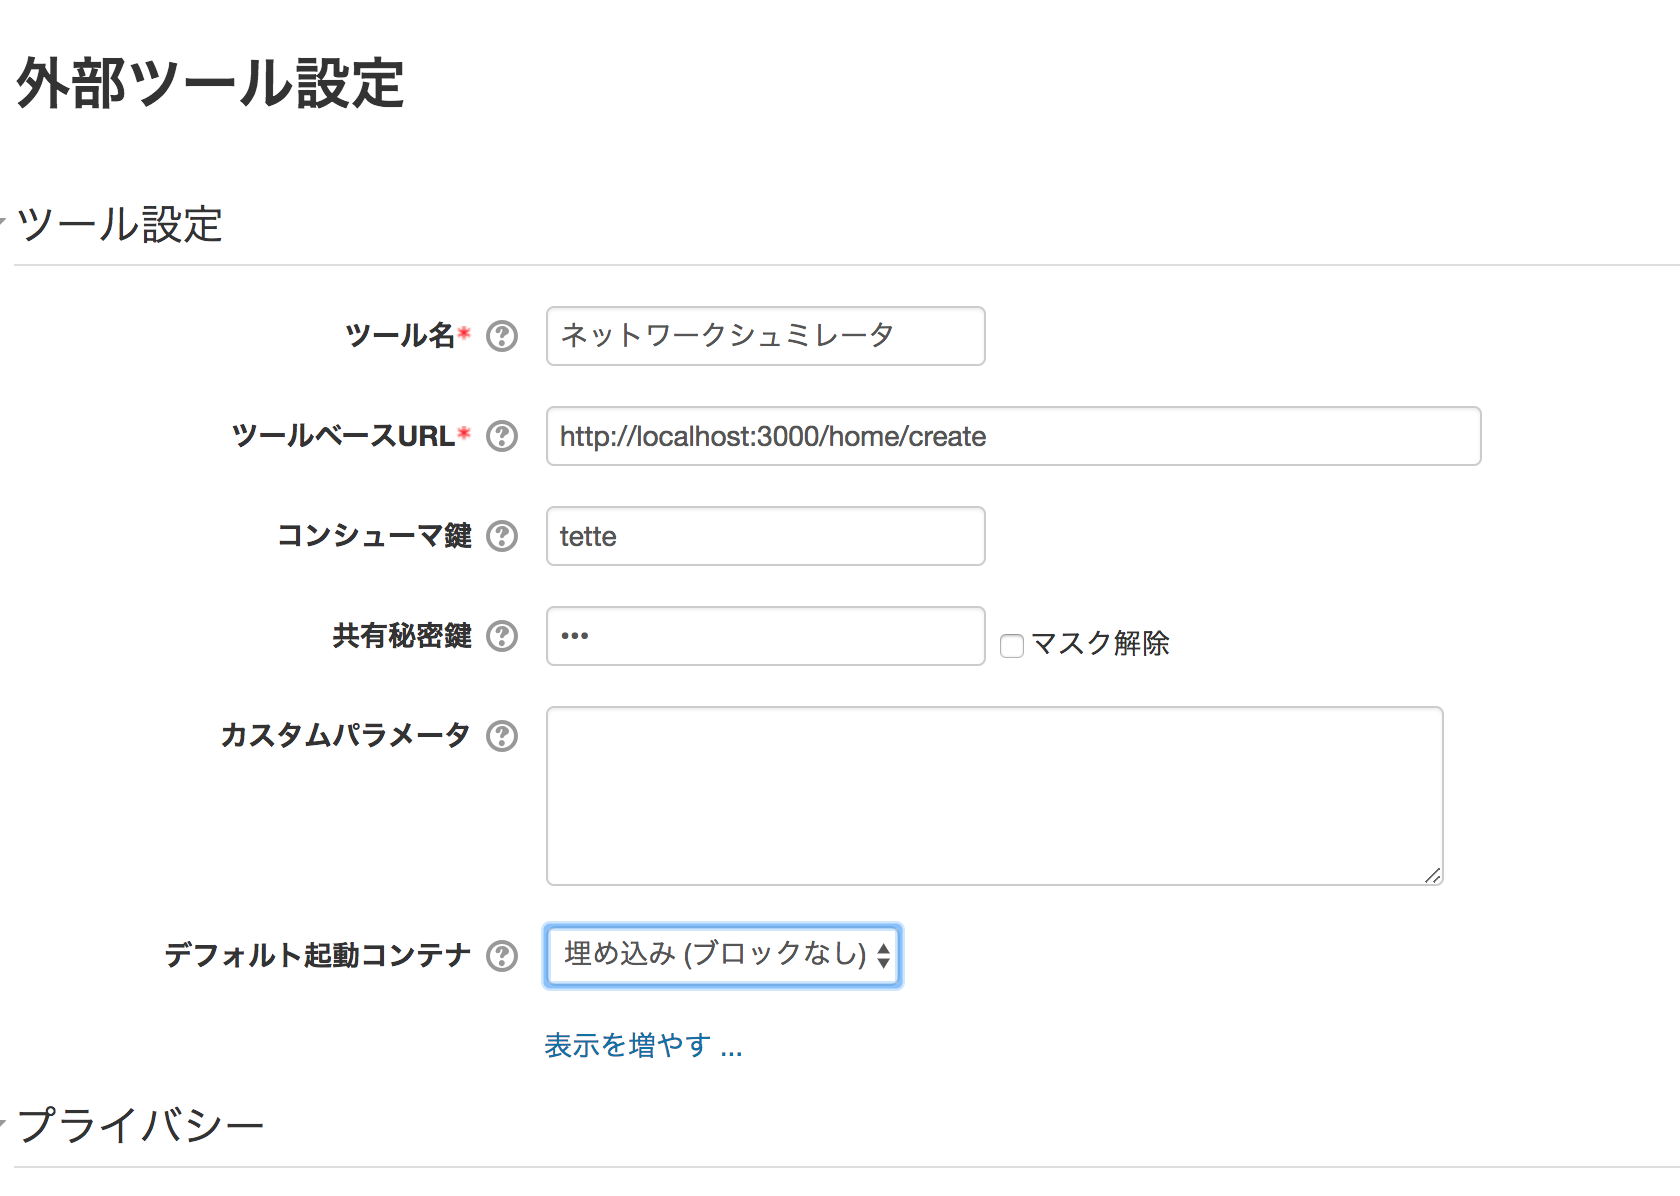
\includegraphics[clip,width=12.0cm,height=8.0cm]{img/moodleSet.png}
    \caption{moodle 外部ツール設定画面}
    \label{fig:moodle config}
  \end{center}
\end{figure}

\begin{figure}[htbp]
  \begin{center}
    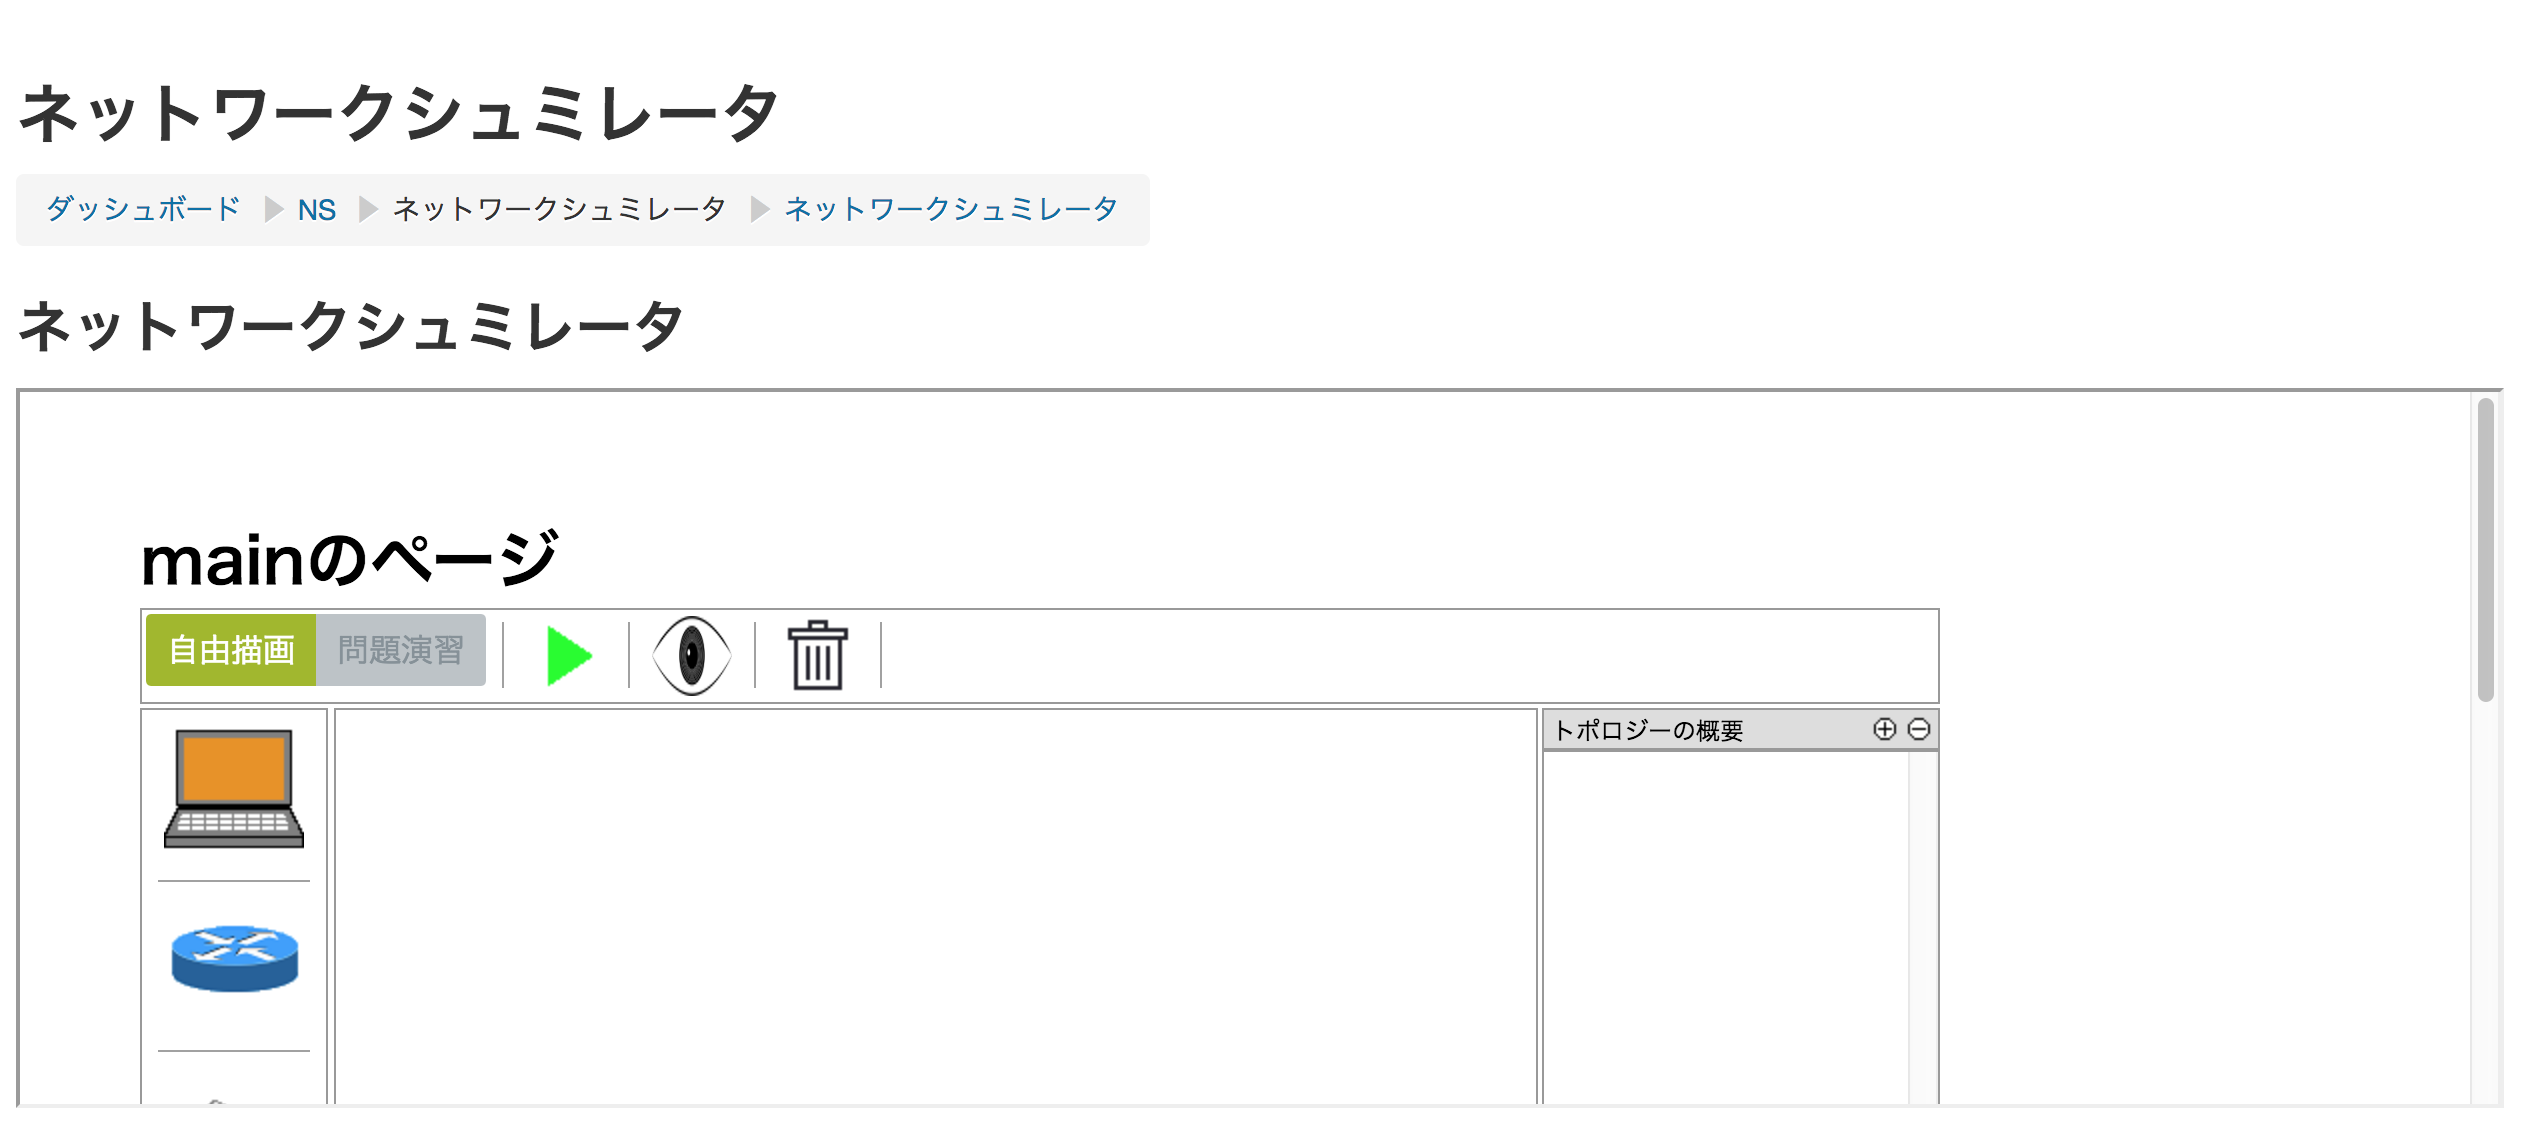
\includegraphics[clip,width=12.0cm,height=8.0cm]{img/LTIstart.png}
    \caption{moodle 外部ツール起動}
    \label{fig:moodle kidou}
  \end{center}
\end{figure}
また、ツール・プロバイダとツール・コンシューマとの間では、OAuthを用いて認証を行っている。\\
\subsection{OAuth}
OAuth(オーオース)とは、SNSやWebサービス間で「アクセス権限の認可」を行うためのプロトコルである。これにより、外部ツールへアクセスする際、ユーザIDとパスワードによる認証を行わずに外部ツールへのアクセスを行うことを可能にしている。また、OAuthには1.0と2.0が存在しているが、本研究ではLTI1.0の実装にあたりOAuth1.0を使用している。
\subsection{OAuth1.0実装手順}
OAuth1.0実装にあたり、OAuth signatureを作成する関数をRubyで自作した。\\
OAuth signatereの作成手順を以下に示す。\\
1.「キー」を作成\\
2.「データ」の作成\\
3.「キー」と「データ」用いてsignatureを作成aaa\\
\subsubsection{キーの作成}
「oauth\_consumer\_secret」、「oauth\_token\_secret」をURLエンコードし、&で繋げれば完成。\\
本研究では「oauth\_consumer\_secret」を設定し、「oauth\_token\_secret」は存在させなかった。また、各々をCGI.escapeによりURLエンコードし、「oauth token secret」を空白とし、&のみを繋げてKeyを作成した。
\subsubsection{データの作成}
1.パラメータをアルファベット順に並べ、キー=値...の形で並べた上で,URLエンコードする。\\
2.リクエストメソッド、リクエストURLをCGI.escapeによりURLエンコードする。\\
3.リクエストメソッド、リクエストURL、パラメータの順で&で繋げることでデータを作成した。\\
\subsubsection{Oauth signatureの作成}
\subsection{成績反映}
成績反映の手順を以下に示す。\\
ツール・コンシューマから送られてくる「SourcedId」取得し、XML内の「SourcedId」を書き変え、ツール・プロバイダでまとめた点数をXML内の「textString」に加えた上で送信する。(沼田と連携した画像を今後貼ります)\\
\begin{figure}[htbp]
  \begin{center}
    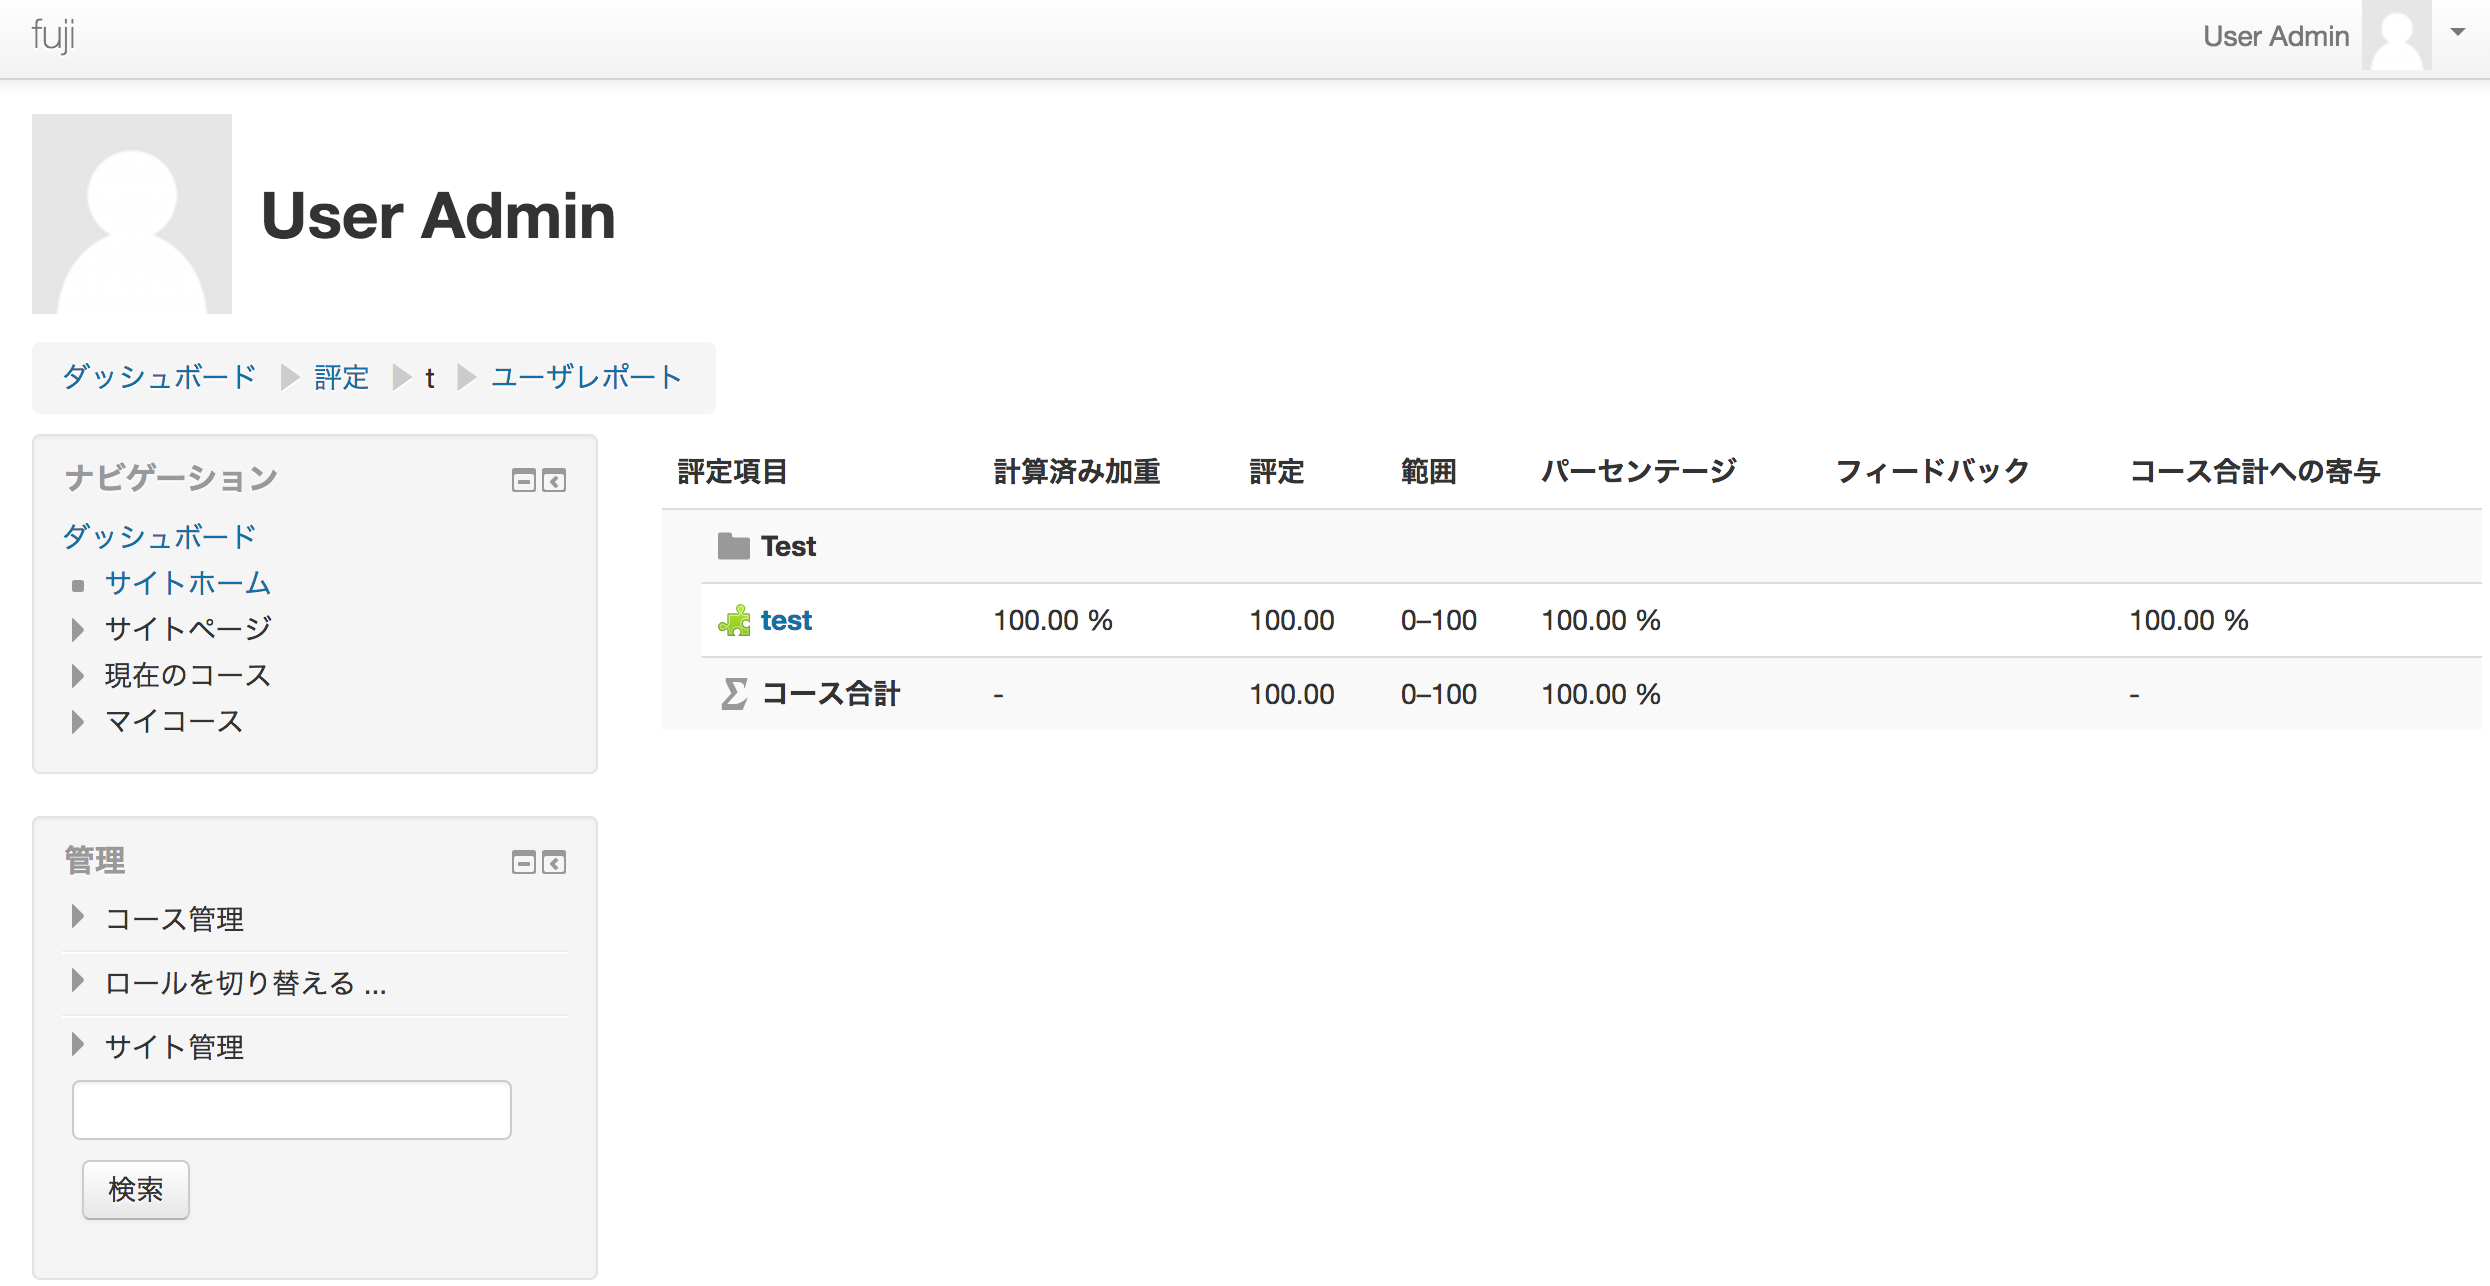
\includegraphics[clip,width=12.0cm,height=8.0cm]{img/score.png}
    \caption{moodle 成績反映}
    \label{fig:moodle score}
  \end{center}
\end{figure}

%\section{まとめと課題}

%\section{まとめと課題}

%\section{まとめと課題}

\input{source/OAuth}
\clearpage

%システムについて
\section{システム概要}
%機能について
\subsection{システム}
\label{tag:function}
本研究では、プラグインとしてLMS上に新しい機能を提供するのではなく、LTIに準拠したWebアプリケーションを用いて、異なるLMSで同様の機能が提供でき、Webアプリケーション側での操作に対しLMS側に特定の点数を返すことを目的とした。そこで、異なる仮想マシン上にそれぞれLMSであるCanvas、Moodleと、独立したWebアプリケーションとしてネットワーク自己学習機能を導入した。また、ネットワーク自己学習機能はRuby on Railsを用いて実装した。これらは図\ref{fig:virtualMachine}で表しているようにネットワーク自己学習機能は実際には独立したWebアプリケーションであるが、あたかもLMS側にプラグインとして導入されているように機能を提供する。

\begin{figure}[htbp]
  \begin{center}
    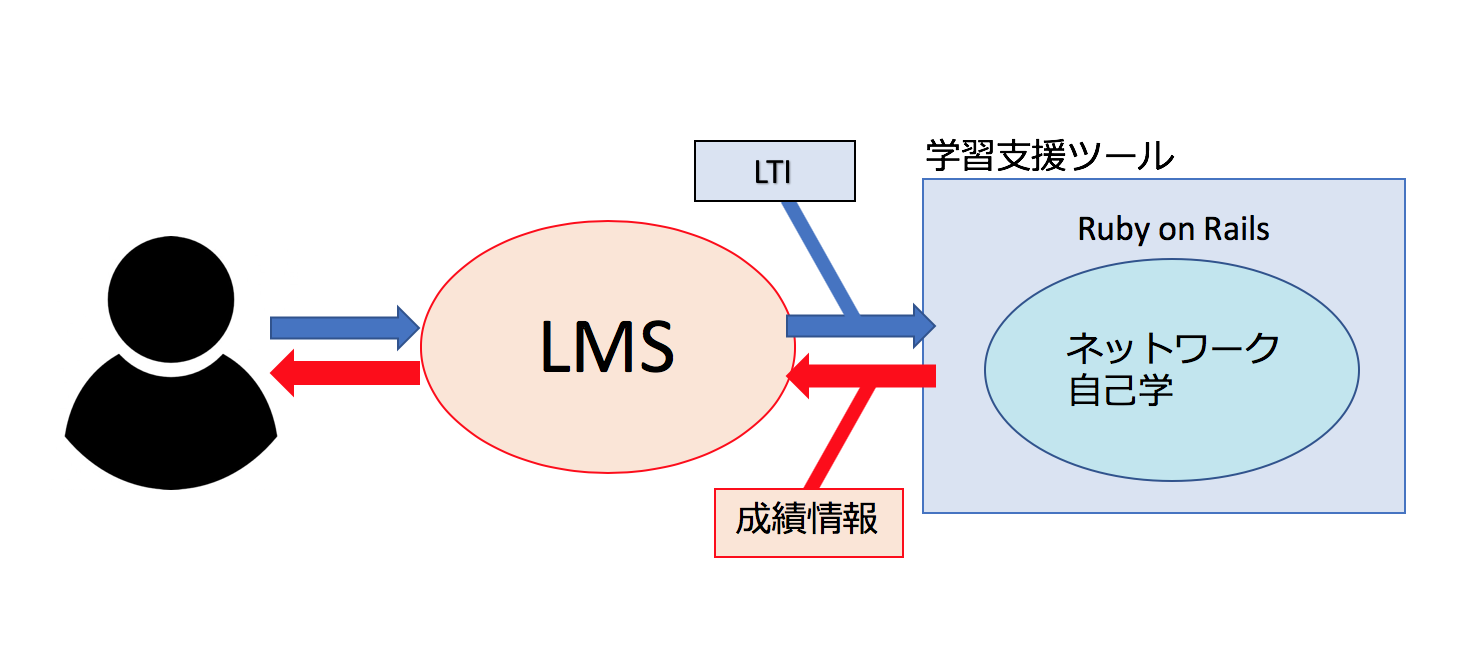
\includegraphics[clip,width=12.0cm,height=8.0cm]{img/system.png}
    \caption{本研究で提案するシステムの構成}
    \label{fig:virtualMachine}
  \end{center}
\end{figure}



また、Webアプリケーション側はLMSに呼び出された際、独立したWebアプリケーションとしてネットワーク自己学習機能を提供する。この機能にはネットワークを自由に構成し、機器情報を設定することのできる自由描画モードと、予め問題として構成されたネットワークに正しい機器情報を追加することで正しいネットワークの作成を目指す問題演習モードが有る。問題演習モードでの正誤によって得られた得点をLMS側に返すことでLMSでの学習者の評価を行う。\\
魚本ら[1]の制作したネットワーク自己学習機能はMoodleの独自プラグインとしてネットワーク自己学習機能を実装している。
クライアントサイドである独自プラグインとしてのシミュレータ部分はHTMLとJavaScriptで、Moodleのプラグインとしての設定の部分はPHPで、シミュレータで作成されたネットワークの構成の正誤の判定プログラムはRubyでそれぞれ記述されている。これは、様々なシステムを使用しているため、複数のシステム間でデータのなどの連携を行わなければならず、安定性にかけていた。\\
 そこで、本研究ではすべてのシステムをRuby on Railsの中で実装した。MVCアーキテクチャに基づいて設計することにより、魚本[1]らのシステムをすべてRuby on Rails内で実現した。これにより、複数のシステム間でのデータの送受信などを行う必要性がなくなり、システムとしての安定性を実現した。

%Ruby on Rails について
\subsection{Ruby on Rails}
\label{tag:rails}
本研究で提案したネットワークシミュレータは、Ruby on Railsを用いて実装されている。Ruby on Railsとは、Rubyで構築された、Webアプリケーションを開発するためのフレームワークである。特徴としてMVCアーキテクチャの採用や設定より規約という設計哲学などが挙げられる。
 MVCとは「Model」「View」「Controller」の頭文字であり、MVCアーキテクチャとはアプリケーションの構成が以下の図\ref{fig:MVC}のようになることに由来している。

\begin{figure}[htbp]
  \begin{center}
    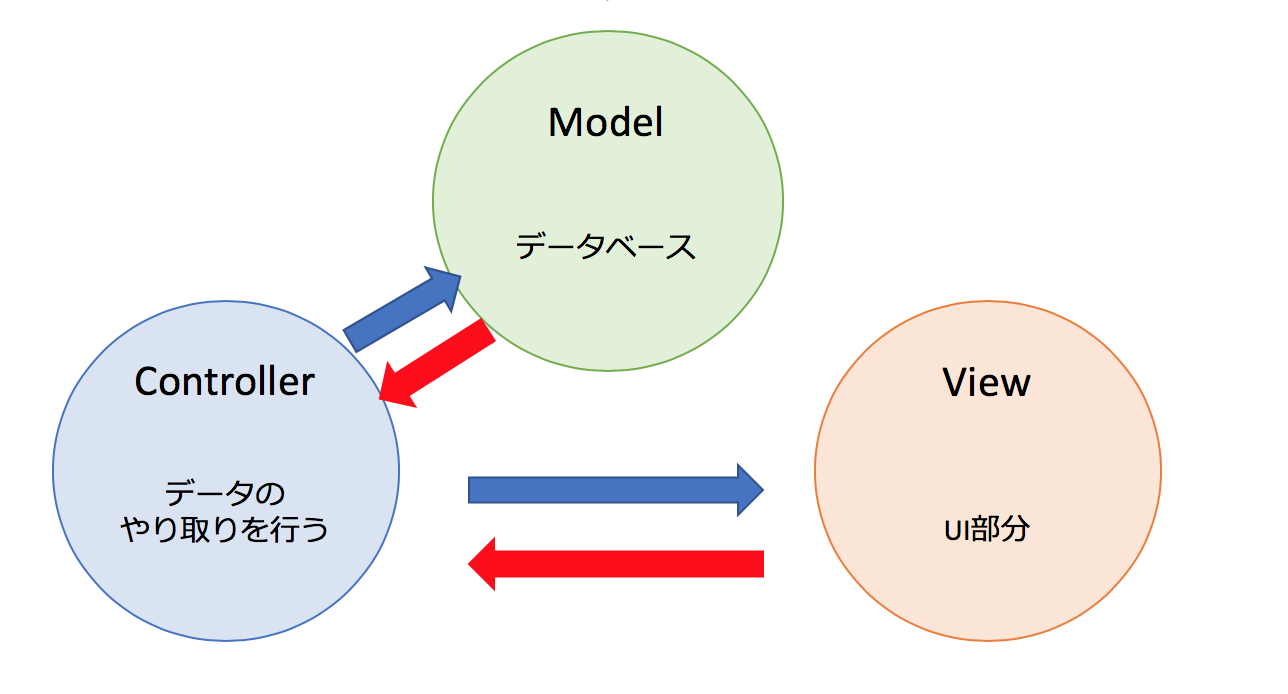
\includegraphics[clip,width=12.0cm,height=8.0cm]{img/mvc.png}
    \caption{MVCアーキテクチャ(いい感じの画像)}
    \label{fig:MVC}
  \end{center}
\end{figure}

%UIについて
\subsection{UIについて}
\label{tag:ui}
UIの基本的な部分は、魚本、大須賀、中村(2018)らの制作したネットワークシミュレータを採用した。これの概要を図\ref{fig:simu}に示す。

\begin{figure}[htbp]
  \begin{center}
    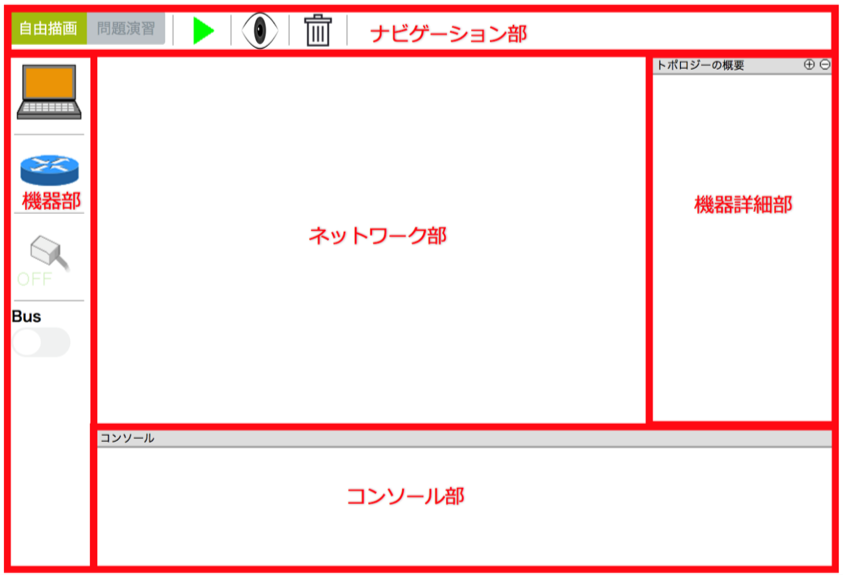
\includegraphics[clip,width=12.0cm,height=8.0cm]{img/simu.png}
    \caption{ネットワークシミュレータ UI(差し替えます)}
    \label{fig:simu}
  \end{center}
\end{figure}

図\ref{fig:simu}のネットワークシミュレータは、実際にネットワークに関する学習を終えた学生に対しアンケートを行い、9割以上の学生がデザインについて見やすいと答えていた。これにより図\ref{fig:simu}のネットワークシミュレータのUIは変更する必要性がないと判断した。
 図\ref{fig:simu}は5つの部分に分けられており、機器部、ナビゲーション部、ネットワーク部、機器詳細部、コンソール部となっている。また、図\ref{fig:simu}では自由描画モードと問題演習モードの2つのモードが用意されている。自由描画モードの際、ナビゲーション部ではそれぞれのアイコンをクリックすることでモードの変更、構築したネットワークの正誤の判定、それぞれの機器の詳細情報の確認、すべての要素の削除を行うことができる。問題演習モードの際は、これに加え練習問題一覧の表示、現在の状況のセーブ、セーブした状態のロード、問題演習モードの終了を行うことができる。機器部では自由描画モードの際にPCやルータをネットワーク部にドロップし、LANをそれぞれつなげることで自由にネットワークを構築することができる。ネットワーク部では構築されているネットワークのそれぞれの機器に必要な情報を追加する事ができる。これによって正しいネットワークを構築していくことが本ネットワークシミュレータの目的である。機器詳細部はネットワーク部で追加されたそれぞれの機器の情報を確認する部分である。コンソール部は不可能な操作やエラーなどの不具合が起こった場合などにそれぞれの理由や結果などをコンソールとして入力される部分である。\\
 これらの機能により、学習者はPCを複数用意し、実際にネットワークを構築することなくネットワークシミュレータ上で擬似的にネットワークの構築を行うことができる。これにより、知識として学習しただけでは分かりづらいネットワークの分野を、視覚的に構築することで実際のネットワークの構成などを理解する助けとなる。

%操作手順について
\subsubsection{操作手順}
\label{tag:operation}

\clearpage

\section{実装実験}
\section{実装試験}
\label{tag:experiment}
本研究ではLTIを用いることで実際に複数のLMSから、独立したWebアプリケーションであるネットワーク自己学習機能を同じように学習支援ツールとして呼び出すことができるのかを確認するために、LTIに準拠したLMSであるMoodle、Canvasを用いての実装実験を行った。\\

%\subsection{LTI使用方法}
LMS上でTool Providerを使用するには、各LMS上で外部ツールの設定を変更する必要がある。例として、moodleでの使用方法を説明する。\\
moodleでは外部ツール設定より、ツール名、ツールURL、コンシューマキー、秘密鍵の設定。これらの設定を得て、moodleからTool Providerを利用することが可能となる。\\
 
%\begin{figure}[htbp]
%  \begin{center}
%    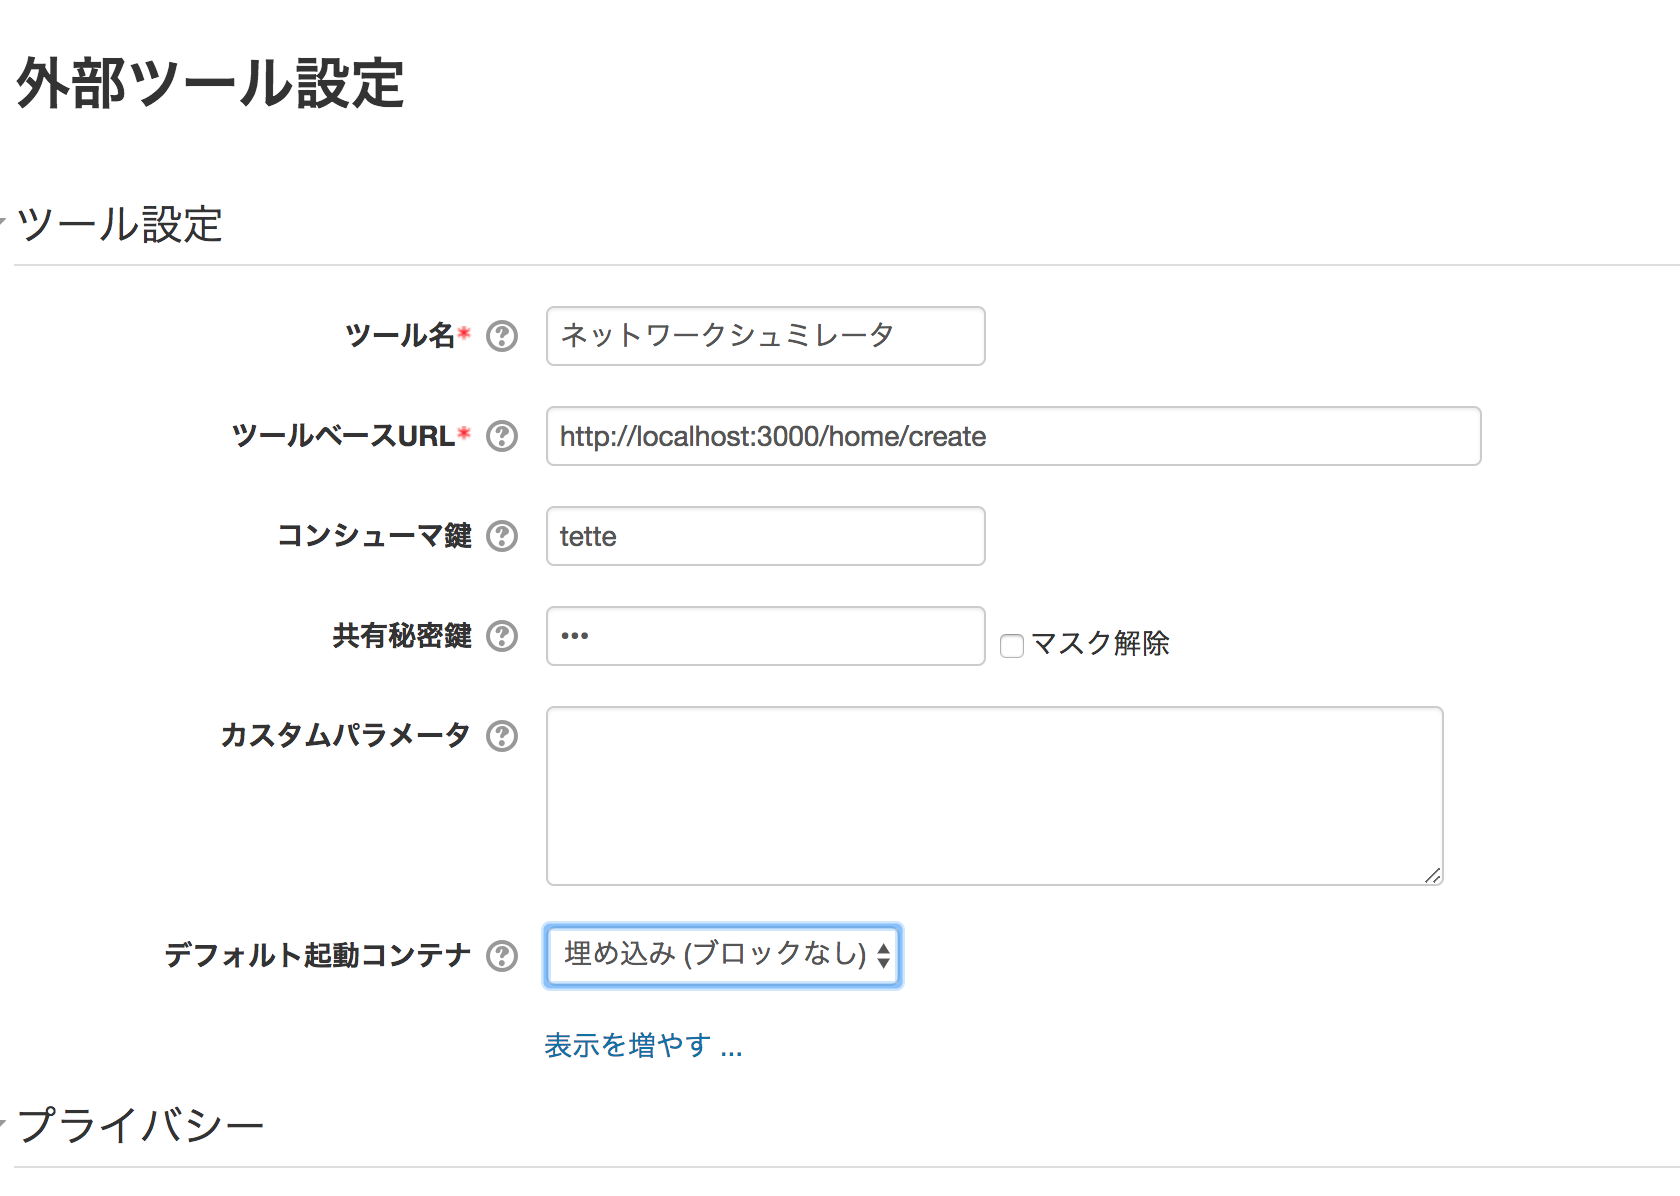
\includegraphics[scale=0.3]{img/moodleSet.png}
%    \caption{moodle 外部ツール設定画面}
%    \label{fig:moodle config}
%  \end{center}
%\end{figure}

%\subsection{成績反映}
Moodleにおいて、実際に成績反映できるかどうかの実験を行った。
%Moodleに置いて、成績の反映ができていることを確認した。
結果を図\ref{fig:moodle score}に示す。
\begin{figure}[htbp]
  \begin{center}
    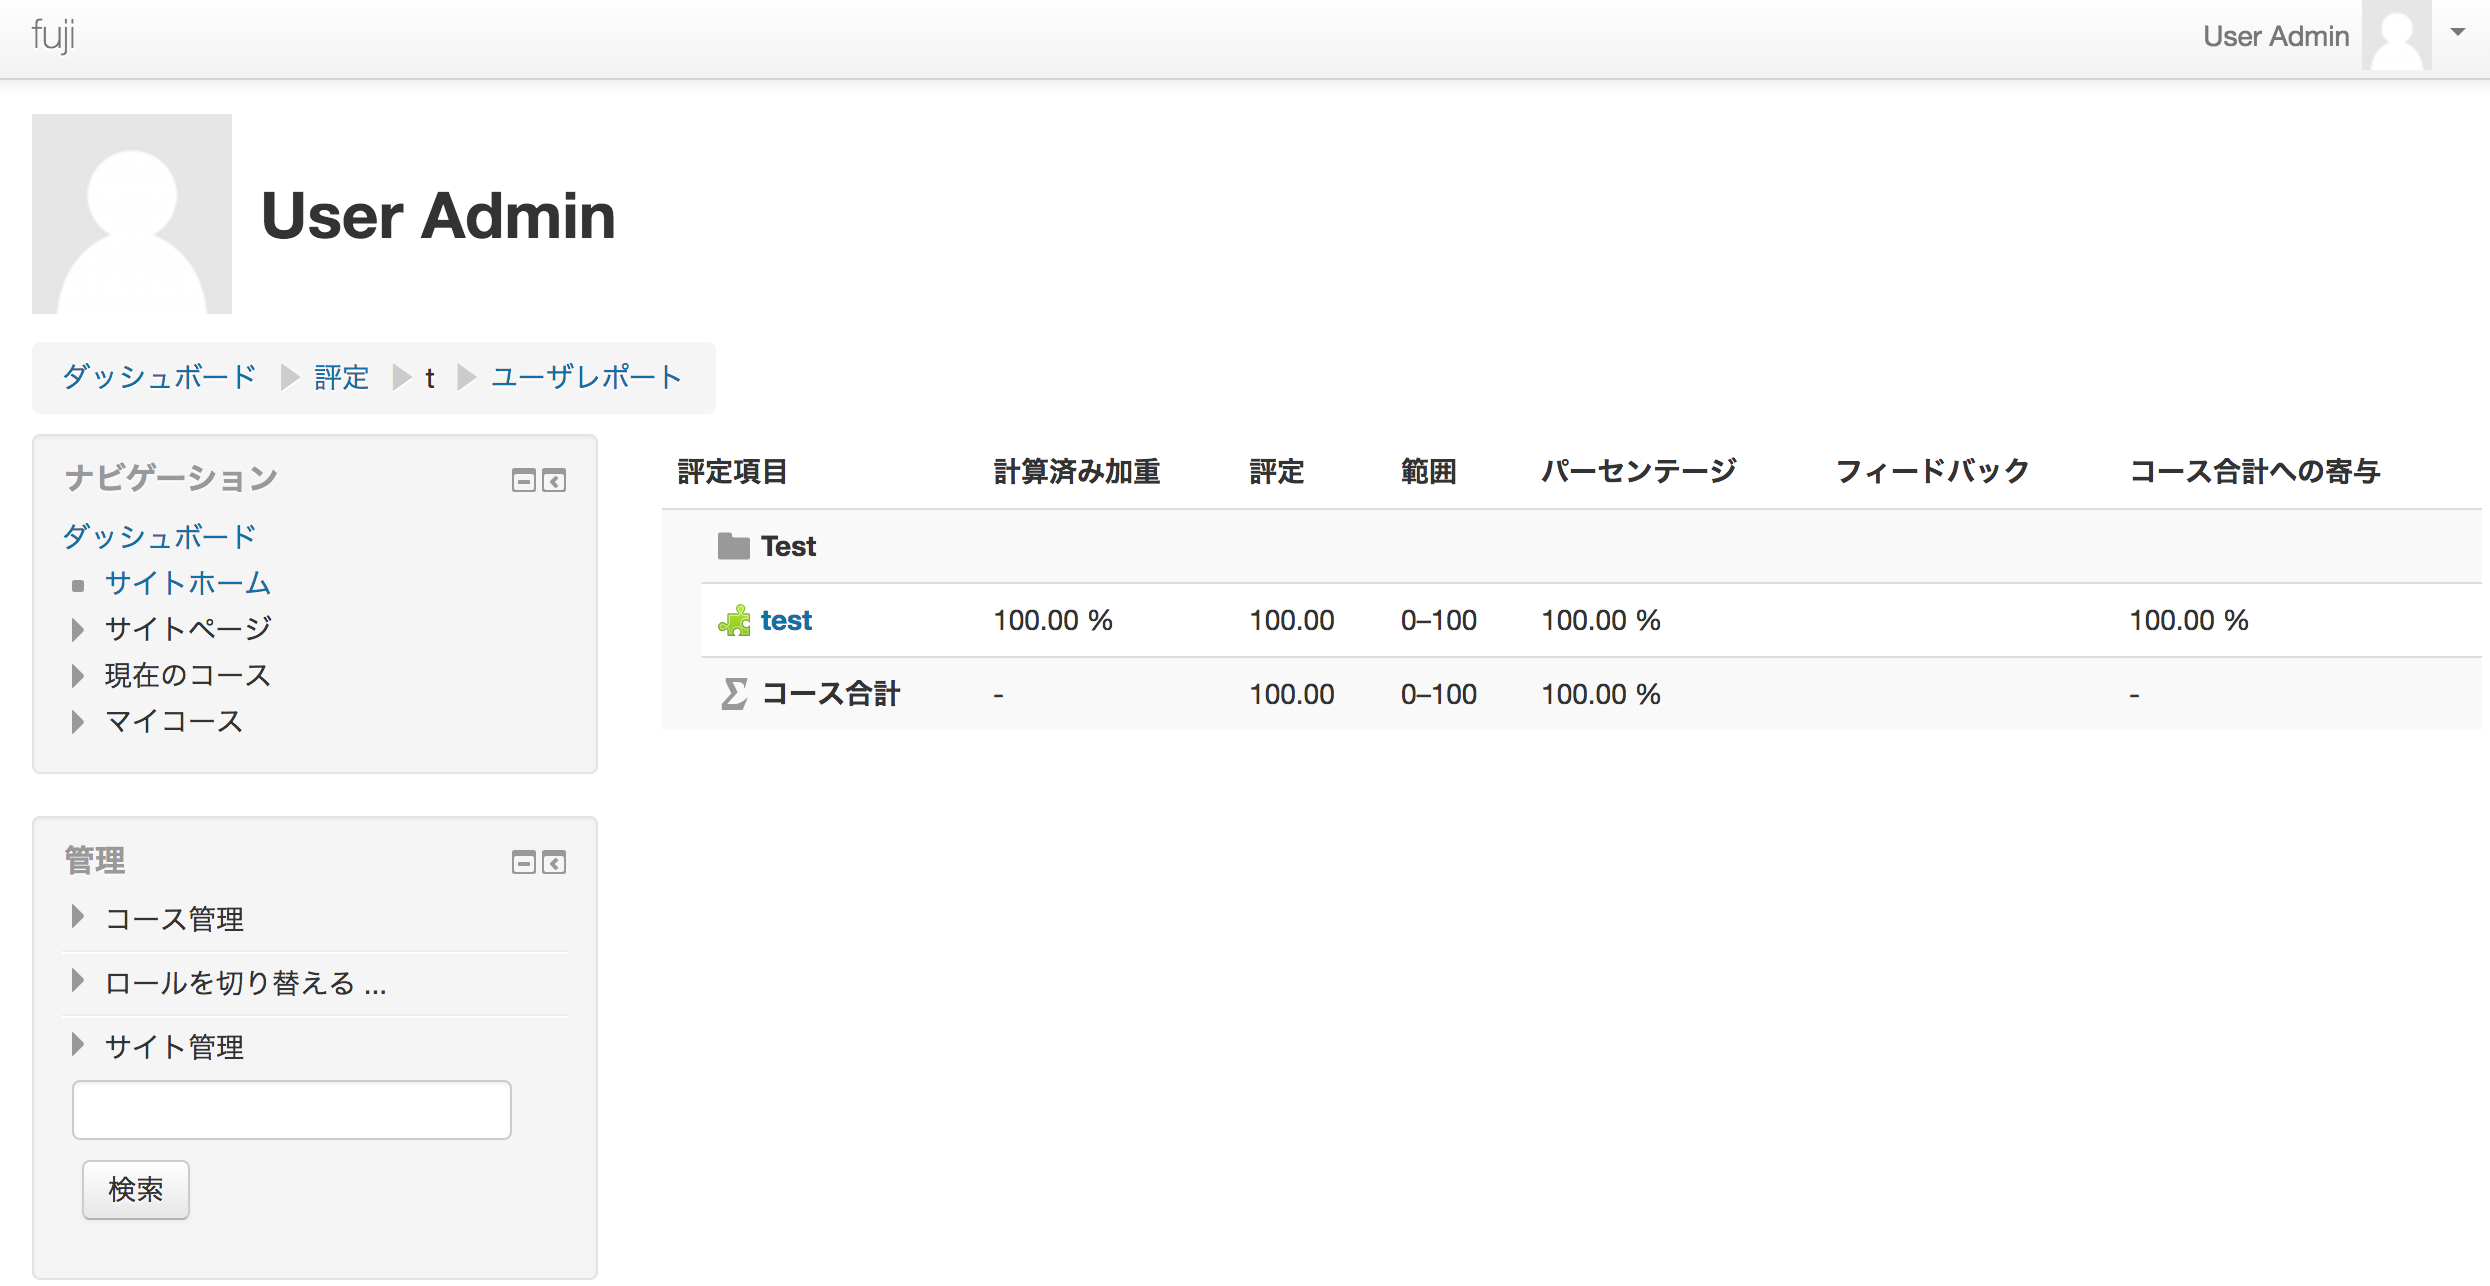
\includegraphics[scale=0.13]{img/score.png}
    \caption{moodle 成績反映}
    \label{fig:moodle score}
  \end{center}
\end{figure}

\clearpage

%まとめと課題
\section{考察}
本研究ではギリシャ神話の系譜図を描画することを目的としているが、
ギリシャ神話は非常に情報が多く複雑な関係が存在しているので、
従来の系譜図表示では関係がわかりにくくなってしまうという問題点がある。
これは\ref{tag:greek}節で挙げた点を解消することで改善がみられると考えられる。
本研究で挙げた問題点のうち線の交わりが増える問題については、
系譜図を3Dで表示することによって解消され、関係の把握をしやすくなったと考えられる。
\cite{ui}において、視覚に入った4〜5個のものの個数を数えずに把握する時間は0.2秒で、
個数が4〜5個を超えると即座の把握は難しくなると記述されている。このことを踏まえると、3Dにしたことのみで
視認性が上がったとは言い難いが、拡大縮小などの機能を使用することでユーザーにとって見やすい情報量に適宜変更することが
できると考えられる。

またアプリケーションの評価をいくつかの質問項目で行っているが、
系譜図はノードの関係を表すグラフであるため、
ユーザがグラフの探索をする際に正しく探索できているかを調査するほかに、
特定のノードまでたどり着くまでの時間を計測することで、
系譜図の探索をスムーズに行えているかどうか数値での評価ができると考えられる。
探索開始から終了までの時間を計測できる機能を付随させることができれば、
より一層システムの改善を行えると期待される。


\section{まとめと課題}
\label{tag:summary}
本研究では、Webブラウザ上でギリシャ神話を元に系譜図を自動で3D描画するシステムを構築した。
本システムでの3D表示により、2D表示では解決できなかった線の交わりと、
複数の婚姻関係・子関係によって系譜図が左右方向に広がることを解消することができた。
また、Webブラウザ上で描画するので特別なソフトウェアを用意する必要はなく、様々な端末で手軽に系譜図を見ることができる。
さらに、マウスを用いて視点を変更することが容易となり、インタラクティブな操作が可能なため利用者が
系譜図をわかりやすく操作することができると期待される。
そして、Webブラウザで答えられるアンケートを作成し利用者からフィードバックを得ることで、
描画システムの改善を図ることができるだろう。

今後の課題としては、親から子への探索、描画はできているが、子から親への探索、
描画ができていないのでわかりやすくするためには解決する必要がある。
また、3Dのため描画された系譜図をマウスを用いて視点変更していくと、
どちらの方向が親方向なのか、子方向なのかわかりにくくなってしまう。
本研究では、アンケートの実施まで至らなかったので、実際にアンケートを取って利用者の意見を参考にして、
描画部分の改善をしていきたいと考える。
アンケートを実施するにあたって、はじめに指定されている人物を見つけ出すことが現状では困難なので、
検索機能を実装し特定の人物を発見しやすくする必要がある。

将来的には、ギリシャ神話の系譜図をより利用者にわかりやすくするために
VRや拡張現実(AR)を利用した系図描画システムを構築することも考えられる。

本研究ではギリシャ神話を対象とした系譜図自動描画を行なったが、
ギリシャ神話以外を対象として関係性の描画をすることもデータベースに情報を持たせることができれば可能であると考える。


% 「UIデザインの心理学」を参考文献として
% 視覚に入った4〜5個のものの個数を数えずに把握する時間は0.2秒で、
% 個数が4〜5個を超えると即座の把握は難しくなる。
% 以上のことから3Dにしたから即座に見やすくなったわけではないが、
% 拡大縮小をすることで自分にとって見やすい情報量に変更することができる。
\clearpage


%謝辞
\section*{謝辞}
本研究での題材となるギリシャ神話の系譜図を提供してくださり、多くの意見をくださった
画家の千葉政助氏、アートフォース株式会社の門山光氏、株式会社画天プロジェクトの井田清氏に、感謝の意を込めて謝辞を送りたいと思います。
また、本研究の御指導や実験への協力をして下さいました藤本准教授とシステム評価研究室の皆様に対し、
ここに心より深く御礼申し上げます。

\clearpages


%参考文献
%key部分に文書中に参考文献として引用する際のラベル名を入れる
\addcontentsline{toc}{section}{参考文献}
\begin{thebibliography}{9999}
  \bibitem{sendai} 魚本裕太,大須賀旭,中村優, "応答性を向上した
IP ネットワーク個人学習システム", 2018.
  \bibitem{kitazawa} 北澤友基, 井口信和, “クラウド環境を利用した IP ネットワーク構築演習支援システムの開発”, 情報処理学会第 74 回全国大会公演論文集, pp.891-892
  \bibitem{moodle} ”Moodle - Open-source learning platform”, \texttt{<https://moodle.org/>},参照2018-12-22
  \bibitem{canvas} “Canvas”, \texttt{<https://www.canvaslms.com/>},参照2018-12-22
  \bibitem{key2} 村上幸生, "Basic LTI に準拠した 学習支援ツールの開発とその評価", 2012
  \bibitem{lti} 「IMS Gloval HP」、\texttt{<https://www.imsglobal.org/specs/ltiomv1p0/specification>}、参照2018-12-22
  \bibitem{ltiw}ウィキペディア OAuth、\texttt{<https://ja.wikipedia.org/wiki/OAuth>}、参照2018-12-22
\end{thebibliography}


\end{document}
